
\subsection{Performance Formula}
\label{sub-sec:formula}
\todo{perf = want and can} \newline

\subsection{PRAE Model}
\label{sub-sec:prae}
\todo{PRAE} \newline

Each person has it's own personality and from a psychological point of view there are different indicator types. One of these indicators are the Myers-Brigs indicator \cite[myers] (based on the research of C. Jung) and offer 8 personality traits that result in 16 personality types. This traits are:
\begin{itemize}
\item extroversion(E) / introversion (I)
\item sensing (S) / intuition(N)
\item thinking (T) / feeling (F) 
\item judgement (J) / perception (P)
\end{itemize}
Each person has one of the two traits from each of the categories above, and the different combination result in 16 possible personalities. Their interpretations can be found at \cite[mbf].

Although the Myers-Brigs indicator was intended to be used by people with no qualifications in psychology, in practice it has proven very difficult for managers to identify the correct traits of their employees without using extensive tests. A simpler model was developed in order to help managers in interacting with their employees based on their personality. 

The \textbf{PRAE} model is based on 4 traits, and as the name suggest the traits are:
\begin{itemize}
\item Person oriented
\item Result oriented
\item Analytical
\item Energetic(motivator)
\end{itemize}

Based on the PRAE model, each parson has a dominant trait that he uses in most situations and is usually the way that a person feels most comfortable to act as. A person also has a secondary trait that he usually uses in unusual/under-pressure situations. At the opposite end there is the adverse trait that hints the behaviour that a person is least comfortable to use.

\begin{figure}[h]
\centering
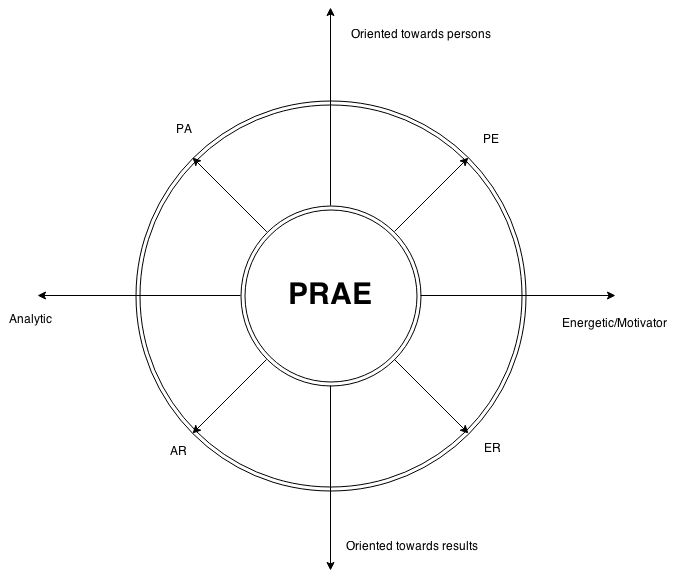
\includegraphics[width=0.8\textwidth]{img/prae.png}
\caption{PRAE personality model}
\label{fig:prae}
\end{figure}

In \ref{fig:prae} the vertical axis (P-R) is called \textit{Scope of action} and the horizontal axis (A-E) is called the \textit{Style of action}. As \ref{fig:prae} hints(although not impossible) the dominant and secondary traits are usually found on different axis. 

Although there are a lot of questionnaires to determine the PRAE model for each person, the dominant and secondary trait can be easily determined by the language that a person uses. In \ref{table:prae} can be found a description of the strong points, weak points and language indicator according to each PRAE trait.

\begin{center}
    \begin{tabular}{ | p{0.11\textwidth} | p{0.3\textwidth} | p{0.3\textwidth} | p{0.29\textwidth} |}
    \hline
    Trait & Strong points & Week Points & Language Indicators \\ \hline
    
    Person oriented 
     &
      \begin{itemize} \itemsep1pt \parskip0pt \parsep0pt
      \item he cares
      \item tactful
      \item motivating
      \item peacemaker, pacifist
      \item looks for cooperation and consensus
      \item tries to involve all the parties
      \end{itemize}
     & 
      \begin{itemize}
      \item easily offend
      \item very emotive
      \item listens to "what the others say"
      \item constantly looking for approval
      \item wishes to please everybody
      \item procrastination in making decisions
      \end{itemize}
     & 
      \begin{itemize}
      \item words like \textit{we, together}
      \item protective vocabulary
      \item do not get straight to the point
      \item spoiled behaviour
      \end{itemize}
     \\ \hline
    Results oriented
     &
     &
     & 
     \\ \hline
    Analytical
     &
     &
     &
     \\ \hline
    Energetic 
     &
     &
     & 
     \\ \hline
    \end{tabular}
    \label{table:prae}
\end{center}




\subsection{RACI Matrix}
\label{sub-sec:raci}
\todo{RACI} \newline

\subsection{FAC Model}
\label{sub-sec:fac}
\todo{FAC feedback} \newline